%prop algorithm methods
\subsubsection*{Algorithm}
To correct for the effect of the bright spots in the image being over bright and the high-key appearance resulting from all the shadows being brightened, we used an algorithm that maps the black and white points of the image to the same value, and adjusts the colours in between to match the target average colour. The algorithm is shown in Equation \ref{eq:prop_algo}.

\begin{equation} \label{eq:prop_algo}
  r' = \left.
  \begin{dcases}
    \displaystyle \Big(\frac{\mean{r_t}}{\mean{r}}\Big)r, & \text{for } r \leq \mean{r} \\
    \displaystyle 255 - 
    \Big(\frac{255 - \mean{r_t}}{255 - \mean{r}}\Big)(255 - r), & \text{for } r > \mean{r} \\
  \end{dcases}
  \right.
\end{equation}

With the same equation applying for the $g$ and $b$ channels.

\subsubsection*{Results}
The complete results are shown in Table \ref{tab:prop_test} in Appendix \ref{app:prop}, a portion is shown here for convenience.

\begin{longtable}{|c||c|c|c|}
    \caption*{Portion of test results of adjusting proportionally based on distance of col or to the average from Table \ref{tab:prop_test} in the Appendix \ref{app:prop}}\\
    \hline
    No. & Original & Target & Results \\
    \hline  \ref{row:prop_test_hand_dark_to_hand_light} &
  \begin{minipage}{.29\textwidth}
    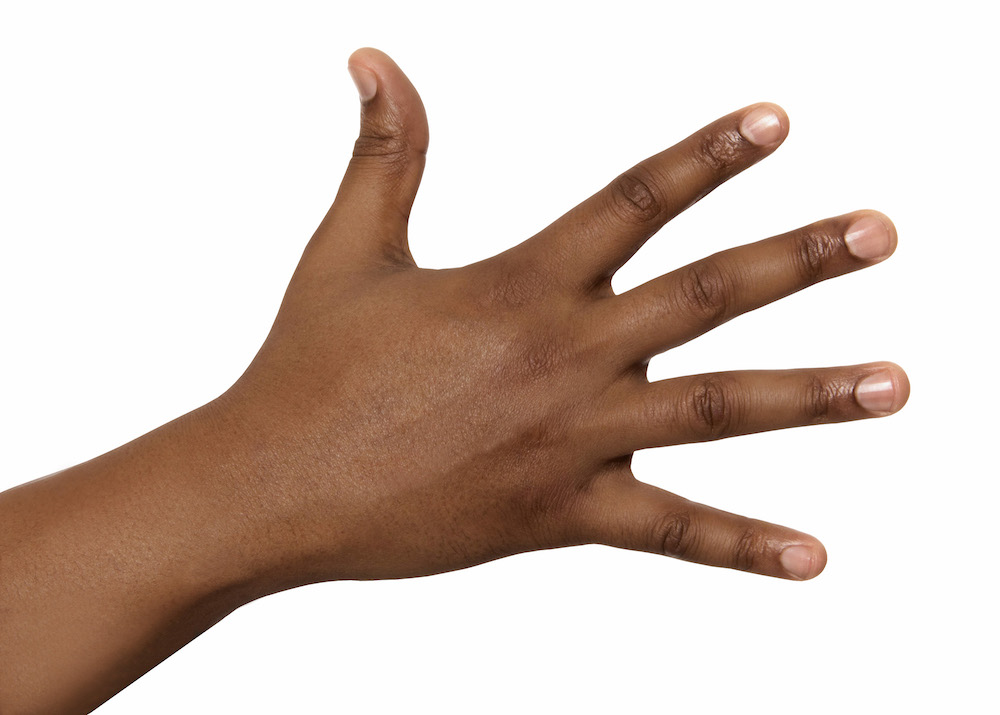
\includegraphics[width=\textwidth,height=\textheight,keepaspectratio]{../inputs/hand_dark.jpg}
  \end{minipage} & 
  \begin{minipage}{.29\textwidth}
    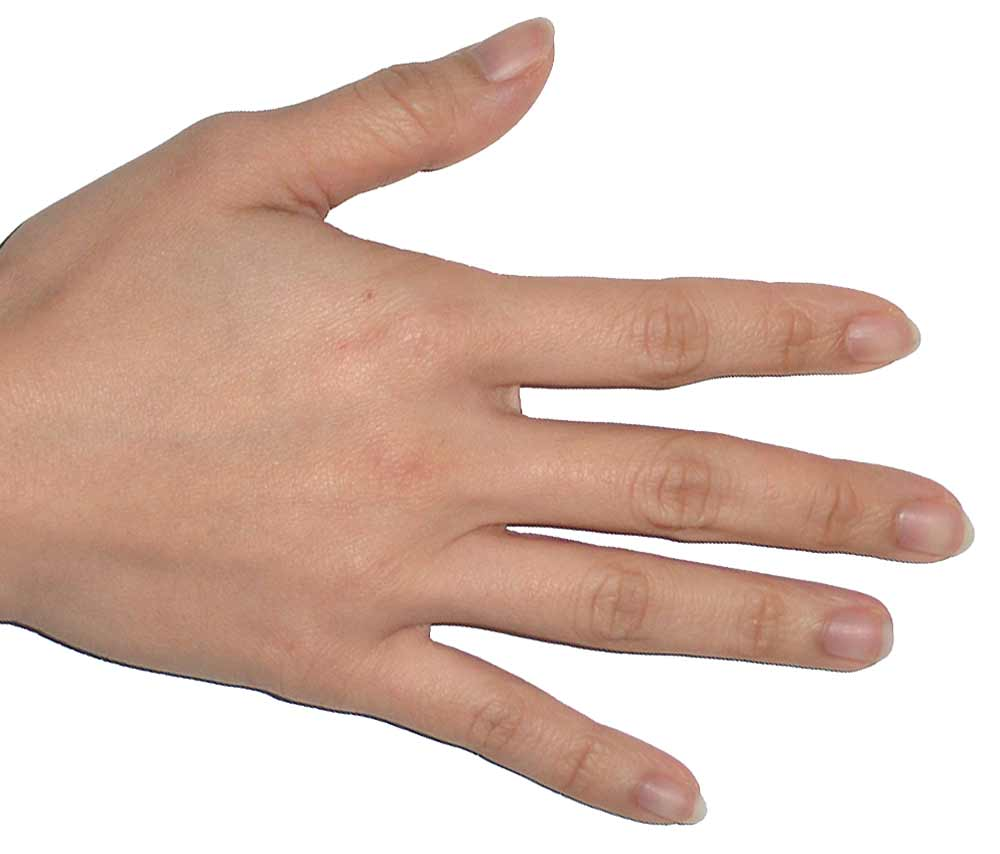
\includegraphics[width=\textwidth,height=\textheight,keepaspectratio]{../inputs/hand_light.jpg}
  \end{minipage} & 
  \begin{minipage}{.29\textwidth}
    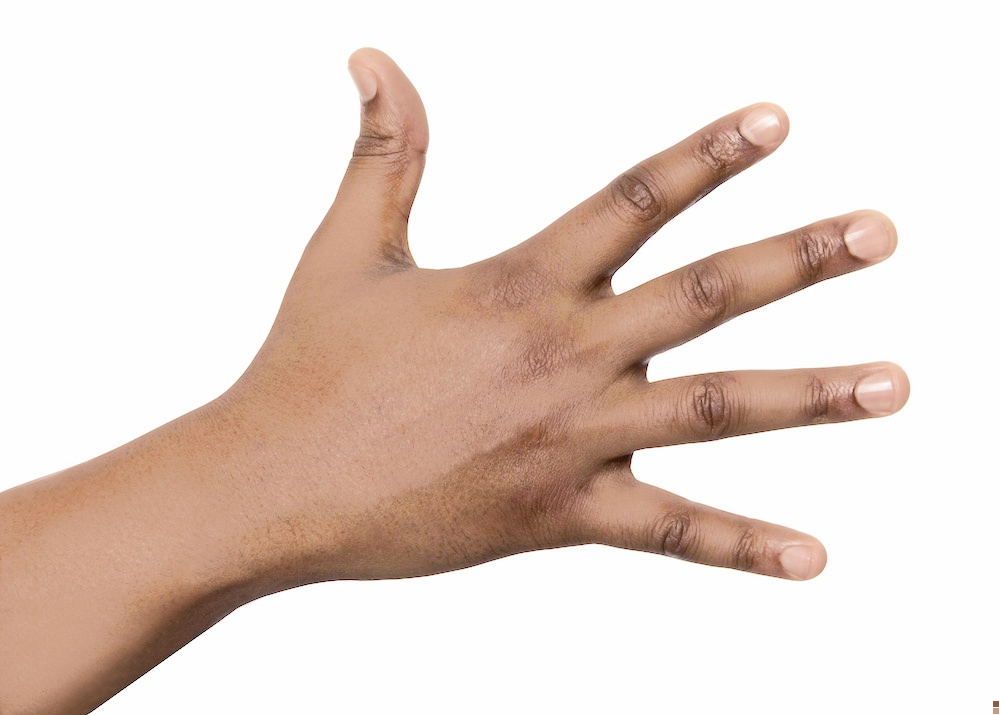
\includegraphics[width=\textwidth,height=\textheight,keepaspectratio]{../rc_test/outputs/20170516_proportional_test/hand_dark_to_hand_light.jpg}
  \end{minipage} \\
    \hline  \ref{row:prop_test_hand_brown_to_hand_dark} &
  \begin{minipage}{.29\textwidth}
    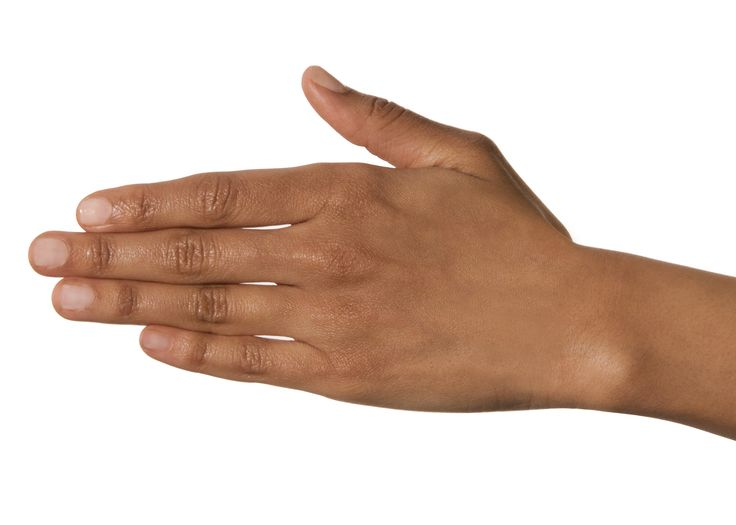
\includegraphics[width=\textwidth,height=\textheight,keepaspectratio]{../inputs/hand_brown.jpg}
  \end{minipage} & 
  \begin{minipage}{.29\textwidth}
    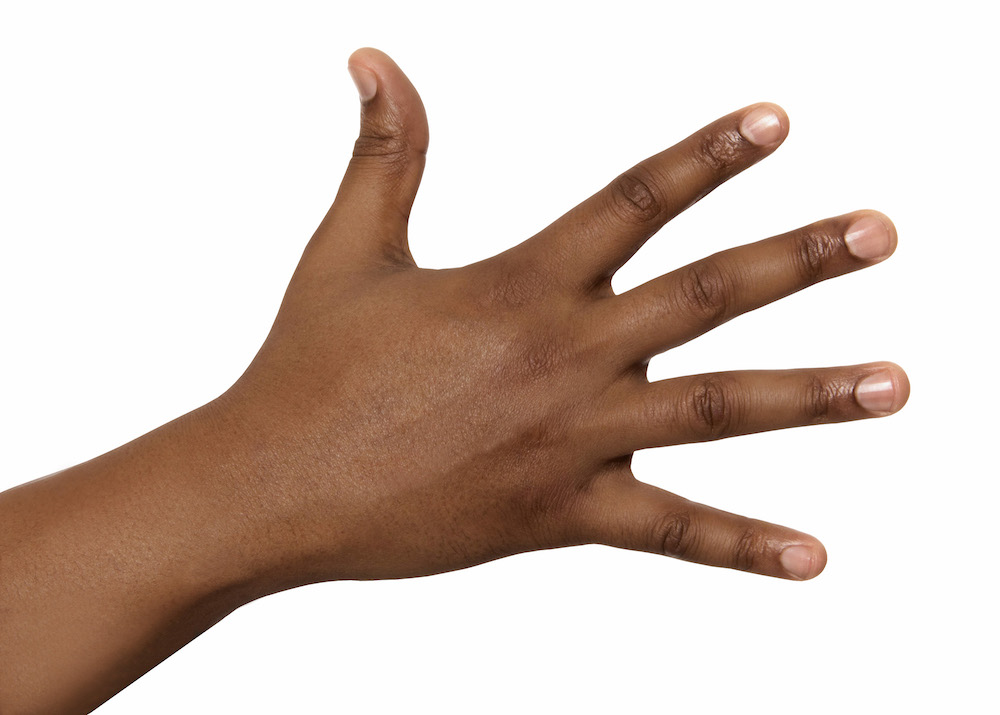
\includegraphics[width=\textwidth,height=\textheight,keepaspectratio]{../inputs/hand_dark.jpg}
  \end{minipage} & 
  \begin{minipage}{.29\textwidth}
    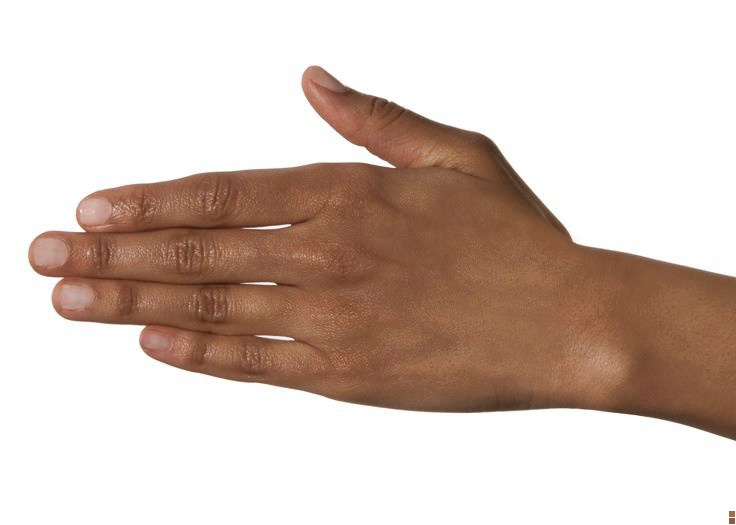
\includegraphics[width=\textwidth,height=\textheight,keepaspectratio]{../rc_test/outputs/20170516_proportional_test/hand_brown_to_hand_dark.jpg}
  \end{minipage} \\
\hline  \ref{row:prop_test_hand_brown_to_hand_light} &
  \begin{minipage}{.29\textwidth}
    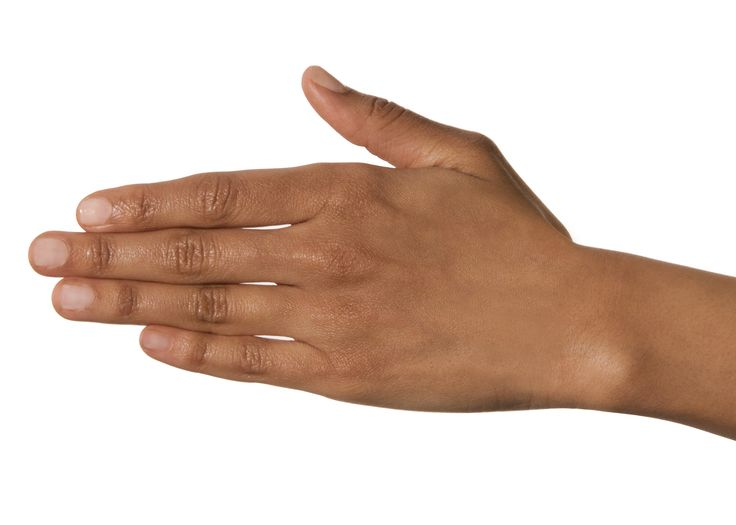
\includegraphics[width=\textwidth,height=\textheight,keepaspectratio]{../inputs/hand_brown.jpg}
  \end{minipage} & 
  \begin{minipage}{.29\textwidth}
    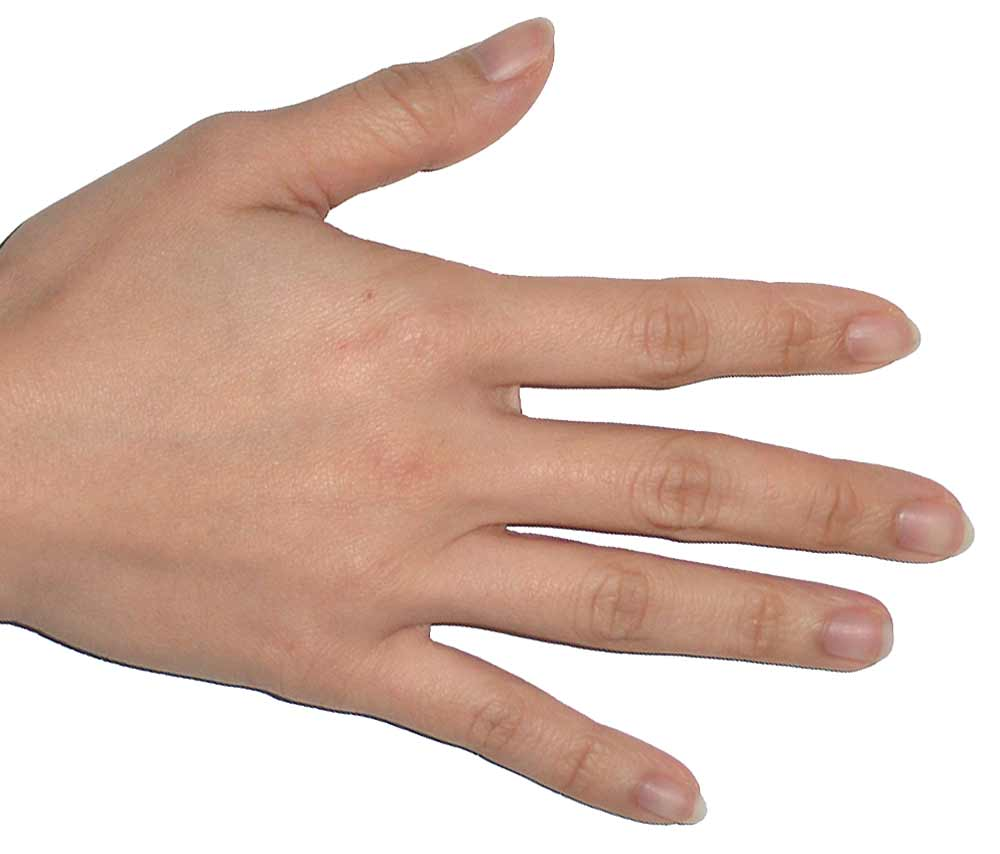
\includegraphics[width=\textwidth,height=\textheight,keepaspectratio]{../inputs/hand_light.jpg}
  \end{minipage} & 
  \begin{minipage}{.29\textwidth}
    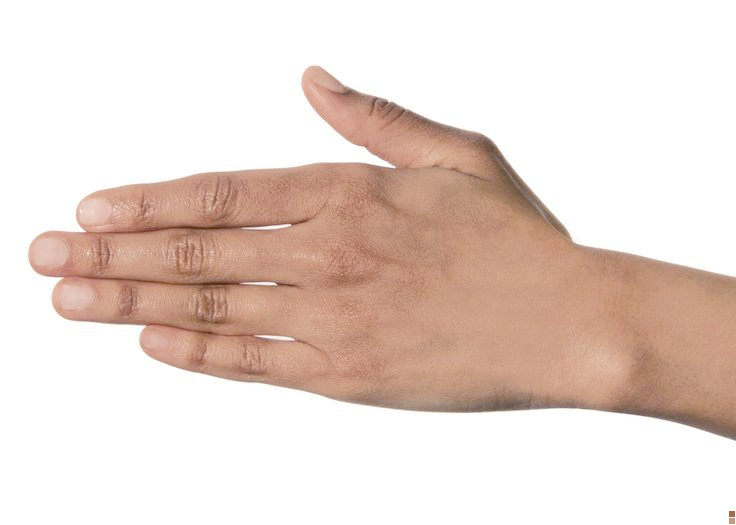
\includegraphics[width=\textwidth,height=\textheight,keepaspectratio]{../rc_test/outputs/20170516_proportional_test/hand_brown_to_hand_light.jpg}
  \end{minipage} \\
  \hline  \ref{row:prop_test_hand_brown_to_hand_pale} &
  \begin{minipage}{.29\textwidth}
    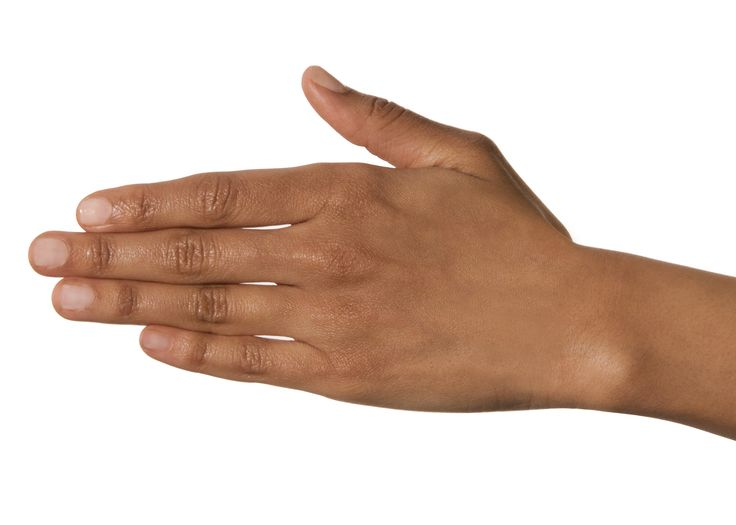
\includegraphics[width=\textwidth,height=\textheight,keepaspectratio]{../inputs/hand_brown.jpg}
  \end{minipage} & 
  \begin{minipage}{.29\textwidth}
    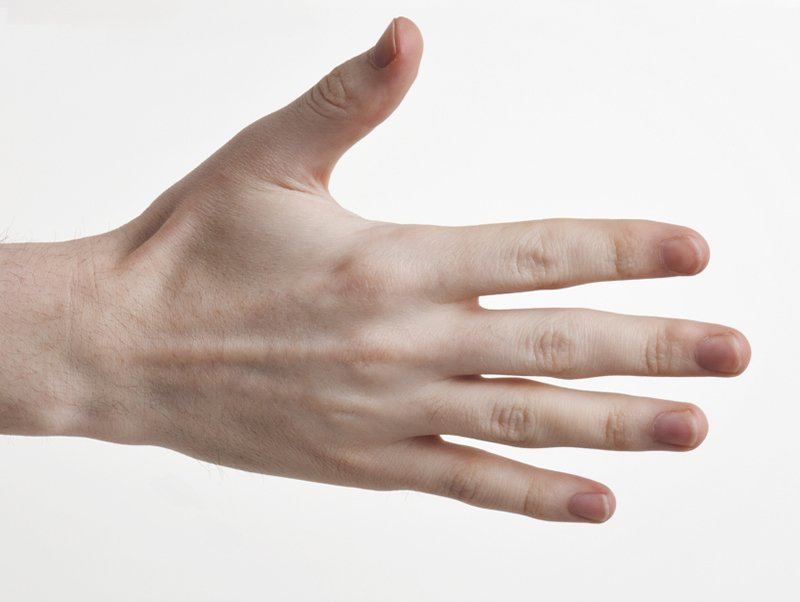
\includegraphics[width=\textwidth,height=\textheight,keepaspectratio]{../inputs/hand_pale.jpg}
  \end{minipage} & 
  \begin{minipage}{.29\textwidth}
    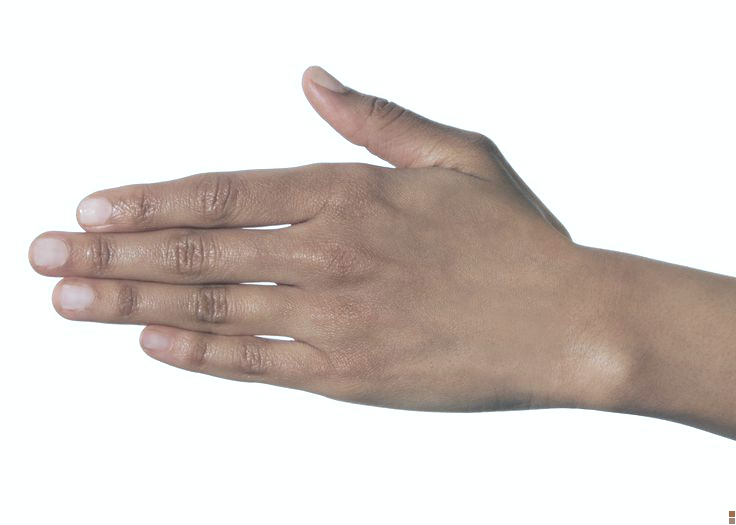
\includegraphics[width=\textwidth,height=\textheight,keepaspectratio]{../rc_test/outputs/20170516_boost_test/hand_brown_to_hand_pale.jpg}
  \end{minipage} \\
    \hline
\end{longtable}

\subsubsection*{Evaluation}
This method improved the appearance of cases with over-bright spots or ``high-key" appearance issues, as Figure \ref{img:compare_bright_spot} shows:
\begin{figure}[H]
    \centering
    \begin{subfigure}[b]{0.40\textwidth}
        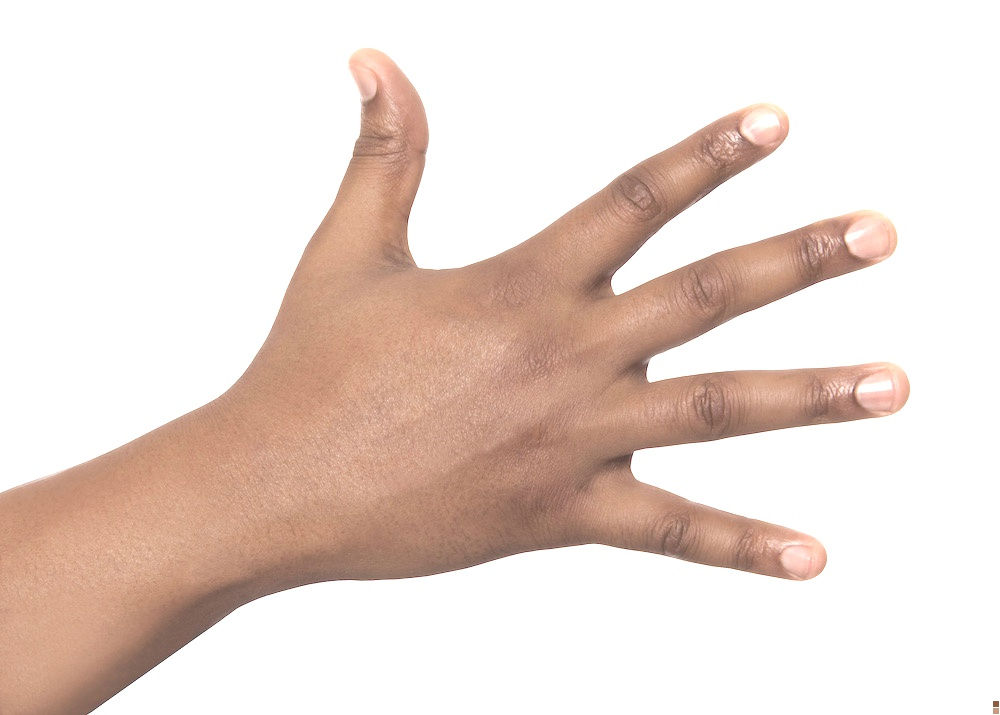
\includegraphics[width=\textwidth]{../rc_test/outputs/20170516_boost_test/hand_dark_to_hand_light.jpg}
        \caption{Simple brightening algorithm result}
    \end{subfigure}
    ~
    \begin{subfigure}[b]{0.40\textwidth}
        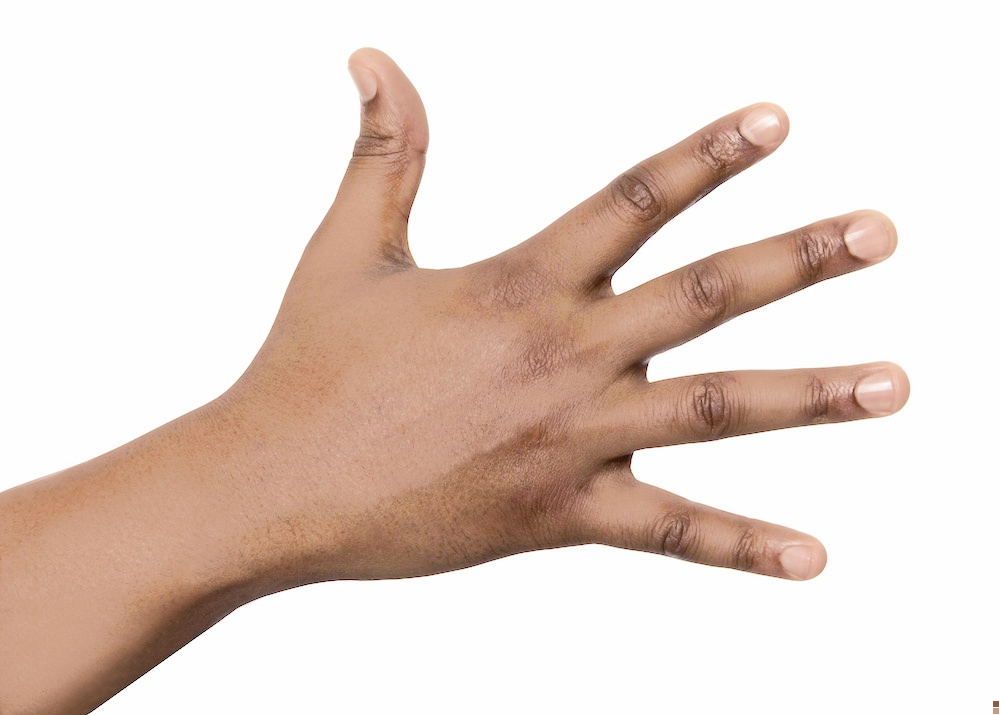
\includegraphics[width=\textwidth]{../rc_test/outputs/20170516_proportional_test/hand_dark_to_hand_light.jpg}
        \caption{Proportional adjustment algorithm result}
    \end{subfigure}
    \caption{Comparison of algorithm \ref{eq:boost_algo} and \ref{eq:prop_algo} results for transforming a dark hand (Figure \ref{img:input_hands_1_dark}) to a light hand (Figure \ref{img:input_hands_1_light}).\label{img:compare_bright_spot}}
\end{figure}

We noted however, that this method noticeably does not correct for, and even exacerbates slightly relative to algorithm \ref{eq:boost_algo}, the dark spots at the joints and creases of a hand of darker skin tone when it is transformed to a lighter skin tone (Row \ref{row:prop_test_hand_brown_to_hand_light}).
